\chapter{Implementación}
El proceso de la implementación así como el desarrollo web del sistema "mesa de servicio", se encuentra principalmente desarrollado en las  versiones de las tecnologías descritas en la siguiente tabla \ref{tab:TecApli}.

  % Table generated by Excel2LaTeX from sheet 'Hoja1'
\begin{table}[H]
	\centering
	\caption{Tecnologías de desarrollo}
	\begin{tabular}{|p{8.145em}|p{9.07em}|}
		\toprule
		\rowcolor[rgb]{ .776,  .878,  .706} \multicolumn{1}{|c|}{\textbf{Tecnología}} & \multicolumn{1}{c|}{\textbf{Versión}} \\
		\midrule
		Sprint Boot & 2.6.3 \\
		\midrule
		MySQL & 8.0.33 \\
		\midrule
		Angular CLI & 15.1.1 \\
		\midrule
		Node.js & 18.13.0 \\
		\bottomrule
	\end{tabular}%
	\label{tab:TecApli}%
\end{table}%

Así pues, para contener un desarrollo estructurado se seguio los principios de SOLID, el cual es una mnemotecnia que hace referencia a 5 principios de diseño para desarrollar software más entendible, flexible y mantenible en un paradigma orientado a objetos, aunque estos no solo aplican a componentes de Software sino también a los servicios.
\newline
Los principios SOLID son los siguientes: 
\begin{itemize}
	
	\item S: Single Responsibility Principle (Una clase debería tener una única función): Una clase debería ser responsable de una única cosa. En el momento en que adquiere más responsabilidad pasa a estar acoplada. 
 \item  O: Open-Closed Principle (Las clases deberían estar abiertas a su extensión, pero cerradas a su modificación): Esencialmente este principio se refiere que si se desea implementar un cambio no soportado, se debería poder implementar sin la necesidad de modificar código, únicamente agregando la nueva funcionalidad. 
\item  L: Liskov Substitution Principle: Tiene como objetivo que una sub-clase pueda asumir el lugar de una superclase sin error. 
\item  I: Interface Segregation Principle (Un cliente no debería estar forzado a depender de métodos que no usa): Establece la restricción de no añadir funcionalidad adicional a las interfaces de modo que acaben teniendo un gran tamaño. Es mejor crear una nueva interfaz y permitir que las clases implementen las interfaces necesarias. 
\item  D: Dependency Inversion Principle (La dependencia debería recaer sobre abstracciones, no sobre clases concretas): Tiene como intención de que las clases de alto nivel no deben depender de clases de bajo nivel.


\end{itemize}
Por lo anterior, el desarrollo del sistema web se encuentra basado en servicios, así como el aprovechar las ventajas que nos ofrece el computo en la nube, tal y como se menciona en la sección \ref{cap:azure}
    \section{Desarrollo del Back End}
    
Los servicios que conforman el Back End, se implementaron aplicando los 5 principios de SOLID, dando como resultado 13 servicios
que cumplen con la calidad de mantenibilidad, eficiencia, dependencia y usabilidad, asi como un marco de desarrollo en el lenguaje Java en su framework Spring Boot, como bien se analizo en la sección \ref{cap:backend} ofrece practicidad para desarrollar servicios.
\newline

Para la elaboración de los servicios, se utilizaron las siguientes dependencias:
\begin{itemize}
 \item JPA (Java Persistence API): Permite persistir nuestro modelo relacional, auto 
generando los queries necesarios para almacenar y consumir la información 
almacenada en las bases de datos.
\item Spring Web: Ofrece características que permiten crear una aplicación web 
consumible.
\item Lombok: Simplifica la creación de Setters, Getters y constructores en una clase de 
datos.

\item Mysql: Es el controlador que permite interconectar los microservicios con la 
base de datos.
\item Model Mapper: Proporciona una solución inmediata para mapear objetos POJO, 
DO y VO.
\item Spring Cloud OpenFeign: Feign facilita la declaración de clientes de servicios 
web.
\item WEB Flux: Nos ofrece anotaciones para implementar aplicaciones reactivas. 

\end{itemize}
\subsection{API de Usuarios Back End}
Objetivo: Gestionar los datos de los usuarios tales como el registro, edición y la obtención de datos personales e inicio de sesión.
\newline
Los endpoint asociados al servicio antes mencionado, son los descritos en la tabla \ref{tab:usuariosend} :
  % Table generated by Excel2LaTeX from sheet 'Hoja1'
\begin{table}[H]
	\centering
	\caption{Endpoint´s de Usuario}
	 \scalebox{0.60}{

\begin{tabular}{|l|c|l|}
	\toprule
	\rowcolor[rgb]{ .267,  .447,  .769} \multicolumn{1}{|c|}{\textcolor[rgb]{ 1,  1,  1}{\textbf{Nombre}}} & \textcolor[rgb]{ 1,  1,  1}{\textbf{Método HTTP}} & \multicolumn{1}{c|}{\textcolor[rgb]{ 1,  1,  1}{\textbf{Path }}} \\
	\midrule
	Guarda Nuevo Usuario & Post & \textcolor[rgb]{ .02,  .388,  .757}{http://heldeskbackend.azurewebsites.net/IPN/helpdesk/Usuario/} \\
	\midrule
	Actualizar Usuario & Put & \textcolor[rgb]{ .02,  .388,  .757}{http://heldeskbackend.azurewebsites.net/IPN/helpdesk/Usuario/} \\
	\midrule
	Listar todas las Usuario & Get & \textcolor[rgb]{ .02,  .388,  .757}{http://heldeskbackend.azurewebsites.net/IPN/helpdesk/Usuario/} \\
	\midrule
	Listar por Usuario & Get & \textcolor[rgb]{ .02,  .388,  .757}{http://heldeskbackend.azurewebsites.net/IPN/helpdesk/Usuario/} \\
	\midrule
	Eliminar por ID Almacen & Delete & \textcolor[rgb]{ .02,  .388,  .757}{http://heldeskbackend.azurewebsites.net/IPN/helpdesk/Usuario/} \\
	\midrule
	Login & Get & \textcolor[rgb]{ .02,  .388,  .757}{http://heldeskbackend.azurewebsites.net/IPN/helpdesk/Usuario/Login/{user}} \\
	\midrule
	Listar Usuario por Username & Get & \textcolor[rgb]{ .02,  .388,  .757}{http://heldeskbackend.azurewebsites.net/IPN/helpdesk/Usuario/userName/{userName}} \\
	\midrule
	Actualizar Contraseña & Put & \textcolor[rgb]{ .02,  .388,  .757}{http://heldeskbackend.azurewebsites.net/IPN/helpdesk/Usuario/actulizar-Password/{user}} \\
	\bottomrule
\end{tabular}%
\label{tab:usuariosend}} %
\end{table}%

\subsection{API de Ticket Back End}
Objetivo: Gestionar los datos de los ticket tales como el registro, edición y eliminación asi como el insumo principal para la operación del “Sistema de Mesa de Servicio”. 
\newline
Los endpoint asociados al servicio antes mencionado, son los descritos en la tabla \ref{tab:ticketend} :

  % Table generated by Excel2LaTeX from sheet 'Hoja1'
\begin{table}[H]
	\centering
	\caption{Endpoint´s de Ticket}
	\scalebox{0.60}{
       \begin{tabular}{|l|c|l|}
     	\toprule
     	\rowcolor[rgb]{ .267,  .447,  .769} \multicolumn{1}{|c|}{\textcolor[rgb]{ 1,  1,  1}{\textbf{Nombre}}} & \textcolor[rgb]{ 1,  1,  1}{\textbf{Método HTTP}} & \multicolumn{1}{c|}{\textcolor[rgb]{ 1,  1,  1}{\textbf{Path }}} \\
     	\midrule
     	Guardar nuevo Ticket & Post & \textcolor[rgb]{ .02,  .388,  .757}{http://heldeskbackend.azurewebsites.net/IPN/helpdesk/Ticket/} \\
     	\midrule
     	Actualizar Tickets  & Put & \textcolor[rgb]{ .02,  .388,  .757}{http://heldeskbackend.azurewebsites.net/IPN/helpdesk/Ticket/} \\
     	\midrule
     	Lista todos los Tickets  & Get & \textcolor[rgb]{ .02,  .388,  .757}{http://heldeskbackend.azurewebsites.net/IPN/helpdesk/Ticket/} \\
     	\midrule
     	Lista de Tickets por ID & Get & \textcolor[rgb]{ .02,  .388,  .757}{http://heldeskbackend.azurewebsites.net/IPN/helpdesk/Ticket/{id\_ticke}} \\
     	\midrule
     	Elimina Tickets  & Delete & \textcolor[rgb]{ .02,  .388,  .757}{http://heldeskbackend.azurewebsites.net/IPN/helpdesk/Ticket/{id\_ticke}} \\
     	\midrule
     	Lista mis Tickets Asigandos & Get & \textcolor[rgb]{ .02,  .388,  .757}{http://heldeskbackend.azurewebsites.net/IPN/helpdesk/Ticket/{id\_user}} \\
     	\midrule
     	Lista mis Tickets Cerrados & Get & \textcolor[rgb]{ .02,  .388,  .757}{http://heldeskbackend.azurewebsites.net/IPN/helpdesk/Ticket/{id\_user}} \\
     	\bottomrule
     
	\end{tabular}%
	\label{tab:ticketend}}%
\end{table}%


\subsection{API de Almacén Back End}
Objetivo: Gestionar los datos y administrar los procesos asociados al stock de refacciones necesarias para la atención de los tickets. 
\newline
Los endpoint asociados al servicio antes mencionado, son los descritos en la tabla \ref{tab:alamcenendp} :
  % Table generated by Excel2LaTeX from sheet 'Hoja1'

\begin{table}[H]
	\centering
	\caption{Endpoint's de Almacén}
	  \scalebox{0.60}{
	\begin{tabular}{|lll}
		\toprule
		\rowcolor[rgb]{ .267,  .447,  .769} \multicolumn{1}{|c}{\textcolor[rgb]{ 1,  1,  1}{\textbf{Nombre}}} & \multicolumn{1}{c}{\textcolor[rgb]{ 1,  1,  1}{\textbf{Metodo HTTP}}} & \multicolumn{1}{c}{\textcolor[rgb]{ 1,  1,  1}{\textbf{Path }}} \\
		\midrule
		\rowcolor[rgb]{ .851,  .882,  .949} Agregar Producto al almacen & Post & \textcolor[rgb]{ .02,  .388,  .757}{http://heldeskbackend.azurewebsites.net/IPN/helpdesk/Almacen/} \\
		\midrule
		Lista Productos  & get  & \textcolor[rgb]{ .02,  .388,  .757}{http://heldeskbackend.azurewebsites.net/IPN/helpdesk/Almacen/} \\
		\midrule
		\rowcolor[rgb]{ .851,  .882,  .949} Lista un producto  & Get  & \textcolor[rgb]{ .02,  .388,  .757}{http://heldeskbackend.azurewebsites.net/IPN/helpdesk/Almacen/{id\_almacen}} \\
		\midrule
		Actualiza producto & Get  & http://heldeskbackend.azurewebsites.net/IPN/helpdesk/Almacen/ \\
		\midrule
		\rowcolor[rgb]{ .851,  .882,  .949} Elimina Producto  & Delete & http://heldeskbackend.azurewebsites.net/IPN/helpdesk/Almacen/{id\_almacen} \\
		\bottomrule
	\end{tabular}%
	\label{tab:alamcenendp}}%
\end{table}%

\subsection{API de Clientes Back End}
Objetivo: Gestionar los datos  tales como el registro, edición y eliminación de los usuarios clientes, los cuales pueden pertenecer a una única cuenta.
\newline
Los endpoint asociados al servicio antes mencionado, son los descritos en la tabla \ref{tab:clienteend} :
  % Table generated by Excel2LaTeX from sheet 'Hoja1'
\begin{table}[H]
	\centering
	\caption{Endpoint's Clientes}
	\  \scalebox{0.60}{
		\begin{tabular}{|l|c|l|}
			\toprule
			\rowcolor[rgb]{ .267,  .447,  .769} \multicolumn{1}{|c|}{\textcolor[rgb]{ 1,  1,  1}{\textbf{Nombre}}} & \textcolor[rgb]{ 1,  1,  1}{\textbf{Método HTTP}} & \multicolumn{1}{c|}{\textcolor[rgb]{ 1,  1,  1}{\textbf{Path }}} \\
			\midrule
			Agregar Cliente & Post & \textcolor[rgb]{ .02,  .388,  .757}{http://heldeskbackend.azurewebsites.net/IPN/helpdesk/Cliente/} \\
			\midrule
			Lista de Clientes completos & Get & \textcolor[rgb]{ .02,  .388,  .757}{http://heldeskbackend.azurewebsites.net/IPN/helpdesk/Cliente/} \\
			\midrule
			Lista de Cliente único & Get & \textcolor[rgb]{ .02,  .388,  .757}{http://heldeskbackend.azurewebsites.net/IPN/helpdesk/Cliente/{id\_cliente}} \\
			\midrule
			Actualizar Cliente & Put & \textcolor[rgb]{ .02,  .388,  .757}{http://heldeskbackend.azurewebsites.net/IPN/helpdesk/Cliente/} \\
			\midrule
			Eliminar Cliente & Delete & \textcolor[rgb]{ .02,  .388,  .757}{http://heldeskbackend.azurewebsites.net/IPN/helpdesk/Cliente/{id\_cliente}} \\
			\bottomrule
		\end{tabular}%
		\label{tab:clienteend}}%
\end{table}%
\subsection{API de Cuenta Back End}
Objetivo: Gestionar los datos asociados a los registros de las cuentas clientes, las cuales son representadas en genera como dependencias de Gobierno.
\newline
Los endpoint asociados al servicio antes mencionado, son los descritos en la tabla \ref{tab:cuentasend} :
  % Table generated by Excel2LaTeX from sheet 'Hoja1'
\begin{table}[H]
	\centering
	\caption{Endpoint's Cuentas}
	  \scalebox{0.60}{
	\begin{tabular}{|l|c|l|}
		\toprule
		\rowcolor[rgb]{ .267,  .447,  .769} \multicolumn{1}{|c|}{\textcolor[rgb]{ 1,  1,  1}{\textbf{Nombre}}} & \textcolor[rgb]{ 1,  1,  1}{\textbf{Método HTTP}} & \multicolumn{1}{c|}{\textcolor[rgb]{ 1,  1,  1}{\textbf{Path }}} \\
		\midrule
		Guardar nueva cuenta & Post & \textcolor[rgb]{ .02,  .388,  .757}{http://heldeskbackend.azurewebsites.net/IPN/helpdesk/Cuenta/} \\
		\midrule
		Lista cuenta única & Get & \textcolor[rgb]{ .02,  .388,  .757}{http://heldeskbackend.azurewebsites.net/IPN/helpdesk/Cuenta/{id\_cuenta}} \\
		\midrule
		Actualizar cuenta & Put & \textcolor[rgb]{ .02,  .388,  .757}{http://heldeskbackend.azurewebsites.net/IPN/helpdesk/Cuenta/} \\
		\midrule
		Lista cuentas & Get & \textcolor[rgb]{ .02,  .388,  .757}{http://heldeskbackend.azurewebsites.net/IPN/helpdesk/Cuenta/} \\
		\midrule
		Eliminar cuenta & Delete & \textcolor[rgb]{ .02,  .388,  .757}{http://heldeskbackend.azurewebsites.net/IPN/helpdesk/Cuenta/{id\_cuenta}} \\
		\bottomrule
	\end{tabular}%
	\label{tab:cuentasend}}%
\end{table}%


\subsection{API de Estados de la República Back End}
Objetivo: Gestionar los datos asociados a los registros de las Entidades federativas que conforman la República Mexicana. 
\newline
Los endpoint asociados al servicio antes mencionado, son los descritos en la tabla \ref{tab:edorepi} :
  % Table generated by Excel2LaTeX from sheet 'Hoja1'
\begin{table}[htbp]
	\centering
	\caption{Endpoint's Estados de la República}
	  \scalebox{0.50}{
	\begin{tabular}{|l|c|l|}

	\toprule
	\rowcolor[rgb]{ .267,  .447,  .769} \multicolumn{1}{|c|}{\textcolor[rgb]{ 1,  1,  1}{\textbf{Nombre}}} & \textcolor[rgb]{ 1,  1,  1}{\textbf{Método HTTP}} & \multicolumn{1}{c|}{\textcolor[rgb]{ 1,  1,  1}{\textbf{Path }}} \\
	\midrule
	Agregar Estados de la República & Post & \textcolor[rgb]{ .02,  .388,  .757}{http://heldeskbackend.azurewebsites.net/IPN/helpdesk/EstadosRepublica/} \\
	\midrule
	Lista  Estados de la República completos & Get & \textcolor[rgb]{ .02,  .388,  .757}{http://heldeskbackend.azurewebsites.net/IPN/helpdesk/EstadosRepublica/} \\
	\midrule
	Lista  Estados de la República único & Get & \textcolor[rgb]{ .02,  .388,  .757}{http://heldeskbackend.azurewebsites.net/IPN/helpdesk/EstadosRepublica/{id\_estadoRepublica}} \\
	\midrule
	Actualizar Estados de la Republica & Put & \textcolor[rgb]{ .02,  .388,  .757}{http://heldeskbackend.azurewebsites.net/IPN/helpdesk/EstadosRepublica/} \\
	\midrule
	Eliminar cuenta & Delete & \textcolor[rgb]{ .02,  .388,  .757}{http://heldeskbackend.azurewebsites.net/IPN/helpdesk/EstadosRepublica/{id\_estadoRepublica}} \\
	\midrule
	Lista  Estados de la República por Región Asignada  & Get & \textcolor[rgb]{ .02,  .388,  .757}{http://heldeskbackend.azurewebsites.net/IPN/helpdesk/EstadosRepublica/{id\_zon}} \\
	\bottomrule
	\end{tabular}%
	\label{tab:edorepi}}%
\end{table}%
\subsection{API de Historial de Asignacion de Ticket Back End}
Objetivo: Gestionar los datos asociados a los registros de la asignacion del ticket a los colaboradores (usuarios), para su atención.
\newline
Los endpoint asociados al servicio antes mencionado, son los descritos en la tabla \ref{tab:edosend}:
  % Table generated by Excel2LaTeX from sheet 'Hoja1'
\begin{table}[H]
	\centering
	\caption{Endpoint's Historial de Asignacion Ticket}
	 \scalebox{0.60}{
	\begin{tabular}{|l|c|l|}
	
	\toprule
	\rowcolor[rgb]{ .267,  .447,  .769} \multicolumn{1}{|c|}{\textcolor[rgb]{ 1,  1,  1}{\textbf{Nombre}}} & \textcolor[rgb]{ 1,  1,  1}{\textbf{Método HTTP}} & \multicolumn{1}{c|}{\textcolor[rgb]{ 1,  1,  1}{\textbf{Path }}} \\
	\midrule
	Agregar Historial de Asignacion & Post & \textcolor[rgb]{ .02,  .388,  .757}{http://heldeskbackend.azurewebsites.net/IPN/helpdesk/HistAsignacion/} \\
	\midrule
	Lista  Historial de Asignacion completos & Get & \textcolor[rgb]{ .02,  .388,  .757}{http://heldeskbackend.azurewebsites.net/IPN/helpdesk/HistAsignacion/} \\
	\midrule
	Lista  Historial de Asignacion único & Get & \textcolor[rgb]{ .02,  .388,  .757}{http://heldeskbackend.azurewebsites.net/IPN/helpdesk/HistAsignacion/{id\_asignacion}} \\
	\midrule
	Actualizar Historial de Asignacion & Put & \textcolor[rgb]{ .02,  .388,  .757}{http://heldeskbackend.azurewebsites.net/IPN/helpdesk/HistAsignacion/} \\
	\midrule
	Eliminar Historial de Asignacion & Delete & \textcolor[rgb]{ .02,  .388,  .757}{http://heldeskbackend.azurewebsites.net/IPN/helpdesk/HistAsignacion/{id\_asignacion}} \\
	\bottomrule
	\end{tabular}%
	\label{tab:edosend}}%
\end{table}%
\subsection{API de Historial de Ticket Back End}
Objetivo: Gestionar los datos asociados a los registros generados cuando se documente o se realice alguna actualización de información al ticket.
\newline
Los endpoint asociados al servicio antes mencionado, son los descritos en la tabla \ref{tab:histtTend} :
  % Table generated by Excel2LaTeX from sheet 'Hoja1'
\begin{table}[H]
	\centering
		\caption{Endpoint's Historial de Asignacion Ticket}
	\scalebox{0.60}{
	\begin{tabular}{|l|c|l|}
		\toprule
		\rowcolor[rgb]{ .267,  .447,  .769} \multicolumn{1}{|c|}{\textcolor[rgb]{ 1,  1,  1}{\textbf{Nombre}}} & \textcolor[rgb]{ 1,  1,  1}{\textbf{Método HTTP}} & \multicolumn{1}{c|}{\textcolor[rgb]{ 1,  1,  1}{\textbf{Path }}} \\
		\midrule
		Agregar al Historial de Ticket & Post & \textcolor[rgb]{ .02,  .388,  .757}{http://heldeskbackend.azurewebsites.net/IPN/helpdesk/HistTicket/} \\
		\midrule
		Lista  Historial de Tickets completos & Get & \textcolor[rgb]{ .02,  .388,  .757}{http://heldeskbackend.azurewebsites.net/IPN/helpdesk/HistTicket/} \\
		\midrule
		Lista  Historial de Ticket único & Get & \textcolor[rgb]{ .02,  .388,  .757}{http://heldeskbackend.azurewebsites.net/IPN/helpdesk/HistTicket/id\_ticket/{id\_ticket}} \\
		\midrule
		Actualizar Historial de Ticket & Put & \textcolor[rgb]{ .02,  .388,  .757}{http://heldeskbackend.azurewebsites.net/IPN/helpdesk/HistTicket/} \\
		\midrule
		Eliminar Historial de Ticket & Delete & \textcolor[rgb]{ .02,  .388,  .757}{http://heldeskbackend.azurewebsites.net/IPN/helpdesk/HistTicket/{id\_historialTicket}} \\
		\bottomrule
	\end{tabular}%
	\label{tab:histtTend}}%
\end{table}%

\subsection{API de Perfiles Back End}
Objetivo: Gestionar los datos asociados a los registros generados para los posibles perfiles con los cuales pueden contar los colaboradores que utilicen el aplicativo.
\newline
Los endpoint asociados al servicio antes mencionado, son los descritos en la tabla \ref{tab:pefil} :
  % Table generated by Excel2LaTeX from sheet 'Hoja1'

\begin{table}[H]
	\centering
			\caption{Endpoint's de Perfiles o Roles}
	\scalebox{0.60}{

\begin{tabular}{|l|c|l|}
	\toprule
	\rowcolor[rgb]{ .267,  .447,  .769} \multicolumn{1}{|c|}{\textcolor[rgb]{ 1,  1,  1}{\textbf{Nombre}}} & \textcolor[rgb]{ 1,  1,  1}{\textbf{Método HTTP}} & \multicolumn{1}{c|}{\textcolor[rgb]{ 1,  1,  1}{\textbf{Path }}} \\
	\midrule
	Agregar Perfil & Post & \textcolor[rgb]{ .02,  .388,  .757}{http://heldeskbackend.azurewebsites.net/IPN/helpdesk/perfil/} \\
	\midrule
	Lista  Perfiles completos & Get & \textcolor[rgb]{ .02,  .388,  .757}{http://heldeskbackend.azurewebsites.net/IPN/helpdesk/perfil/} \\
	\midrule
	Lista  un  único Perfil & Get & \textcolor[rgb]{ .02,  .388,  .757}{http://heldeskbackend.azurewebsites.net/IPN/helpdesk/perfil/{id\_perfil}} \\
	\midrule
	Actualizar Perfil & Put & \textcolor[rgb]{ .02,  .388,  .757}{http://heldeskbackend.azurewebsites.net/IPN/helpdesk/perfil/} \\
	\midrule
	Eliminar Perfil  & Delete & \textcolor[rgb]{ .02,  .388,  .757}{http://heldeskbackend.azurewebsites.net/IPN/helpdesk/perfil/{id\_perfil}} \\
	\bottomrule
\end{tabular}%
		\label{tab:pefil}}%
	\end{table}%

\subsection{API de Servicios al Cliente Back End}
Objetivo: Gestionar los datos  tales como el registro, edición  y edición de los servicios que se proporcionaran a los clientes, asi como la confuracion del SLA con el que contara el servicio.
\newline
Los endpoint asociados al servicio antes mencionado, son los descritos en la tabla \ref{tab:Serviceend} :

  % Table generated by Excel2LaTeX from sheet 'Hoja1'
\begin{table}[H]
	\centering
		\caption{Endpoint's de Clientes}
	\scalebox{0.60}{
	\begin{tabular}{|l|c|l|}
		\toprule
		\rowcolor[rgb]{ .267,  .447,  .769} \multicolumn{1}{|c|}{\textcolor[rgb]{ 1,  1,  1}{\textbf{Nombre}}} & \textcolor[rgb]{ 1,  1,  1}{\textbf{Metodo HTTP}} & \multicolumn{1}{c|}{\textcolor[rgb]{ 1,  1,  1}{\textbf{Path }}} \\
		\midrule
		Guardar nuevo servicio & post & \textcolor[rgb]{ .02,  .388,  .757}{http://heldeskbackend.azurewebsites.net/IPN/helpdesk/Servicios/} \\
		\midrule
		Actualizar Servicios  & Put & \textcolor[rgb]{ .02,  .388,  .757}{http://heldeskbackend.azurewebsites.net/IPN/helpdesk/Servicios/} \\
		\midrule
		Lista todos los servicios  & Get & \textcolor[rgb]{ .02,  .388,  .757}{http://heldeskbackend.azurewebsites.net/IPN/helpdesk/Servicios/} \\
		\midrule
		Lista de Servicios por ID & Get & \textcolor[rgb]{ .02,  .388,  .757}{http://heldeskbackend.azurewebsites.net/IPN/helpdesk/Servicios/{id\_servicio}} \\
		\midrule
		Elimina Servicios  & Delete & \textcolor[rgb]{ .02,  .388,  .757}{http://heldeskbackend.azurewebsites.net/IPN/helpdesk/Servicios/{id\_servicio}} \\
		\bottomrule
	\end{tabular}%
	\label{tab:Serviceend}}%
\end{table}%



\subsection{API de Estatus del Ticket Back End}
Objetivo: Gestionar los datos asociados a los estatus que podrá tomar un ticket en su ciclo de vida.
\newline
Los endpoint asociados al servicio antes mencionado, son los descritos en la tabla \ref{tab:cuenend} :
  % Table generated by Excel2LaTeX from sheet 'Hoja1'
\begin{table}[H]
	\centering
	\caption{Endpoint's de Cuentas}
	\scalebox{0.60}{
	\begin{tabular}{|l|c|l|}
		\toprule
		\rowcolor[rgb]{ .267,  .447,  .769} \multicolumn{1}{|c|}{\textcolor[rgb]{ 1,  1,  1}{\textbf{Nombre}}} & \textcolor[rgb]{ 1,  1,  1}{\textbf{Método HTTP}} & \multicolumn{1}{c|}{\textcolor[rgb]{ 1,  1,  1}{\textbf{Path }}} \\
		\midrule
		Guardar nueva cuenta & Post & \textcolor[rgb]{ .02,  .388,  .757}{http://heldeskbackend.azurewebsites.net/IPN/helpdesk/Cuenta/} \\
		\midrule
		Lista cuenta única & Get & \textcolor[rgb]{ .02,  .388,  .757}{http://heldeskbackend.azurewebsites.net/IPN/helpdesk/Cuenta/{id\_cuenta}} \\
		\midrule
		Actualizar cuenta & Put & \textcolor[rgb]{ .02,  .388,  .757}{http://heldeskbackend.azurewebsites.net/IPN/helpdesk/Cuenta/} \\
		\midrule
		Lista cuentas & Get & \textcolor[rgb]{ .02,  .388,  .757}{http://heldeskbackend.azurewebsites.net/IPN/helpdesk/Cuenta/} \\
		\midrule
		Eliminar cuenta & Delete & \textcolor[rgb]{ .02,  .388,  .757}{http://heldeskbackend.azurewebsites.net/IPN/helpdesk/Cuenta/{id\_cuenta}} \\
		\bottomrule
	\end{tabular}%
	\label{tab:cuenend}}%
\end{table}%

\subsection{API de Zonas o Regiones de la República  Back End}
Objetivo:  Gestionar los datos asociados a las regiones de México las cuales son las zonas geográficas en las que se agrupan las entidades federativas de los Estados Unidos Mexicanos.
\newline
Los endpoint asociados al servicio antes mencionado, son los descritos en la tabla \ref{tab:zonaed} :
  % Table generated by Excel2LaTeX from sheet 'Hoja1'
\begin{table}[H]
	\centering
	\caption{Endpoint's de Zonas o Región}
\scalebox{0.60}{
	\begin{tabular}{|l|c|l|}
		\toprule
		\rowcolor[rgb]{ .267,  .447,  .769} \multicolumn{1}{|c|}{\textcolor[rgb]{ 1,  1,  1}{\textbf{Nombre}}} & \textcolor[rgb]{ 1,  1,  1}{\textbf{Método HTTP}} & \multicolumn{1}{c|}{\textcolor[rgb]{ 1,  1,  1}{\textbf{Path }}} \\
		\midrule
		Guardar nueva Zona o Región & Post & \textcolor[rgb]{ .02,  .388,  .757}{http://heldeskbackend.azurewebsites.net/IPN/helpdesk/ZonaEstado/} \\
		\midrule
		Lista Zona o Región única & Get & \textcolor[rgb]{ .02,  .388,  .757}{http://heldeskbackend.azurewebsites.net/IPN/helpdesk/ZonaEstado/{id\_zona}} \\
		\midrule
		Actualizar Zona o Región & Put & \textcolor[rgb]{ .02,  .388,  .757}{http://heldeskbackend.azurewebsites.net/IPN/helpdesk/ZonaEstado/} \\
		\midrule
		Lista Zona o Región & Get & \textcolor[rgb]{ .02,  .388,  .757}{http://heldeskbackend.azurewebsites.net/IPN/helpdesk/ZonaEstado/} \\
		\midrule
		Eliminar Zona o Región & Delete & \textcolor[rgb]{ .02,  .388,  .757}{http://heldeskbackend.azurewebsites.net/IPN/helpdesk/ZonaEstado/{id\_zona}} \\
		\bottomrule
	\end{tabular}%
	\label{tab:zonaed}}%
\end{table}%


  \section{Desarrollo del Front End}

El desarrollo del Front End se implementó bajo la arquitectura que recomienda el marco 
de trabajo Angular, es decir, toda la aplicación está contenida en distintos módulos los 
cuales permiten que el servidor los renderice por partes al momento de su utilización y no 
completamente desde un inicio.
De igual manera, esta arquitectura sigue el principio “Keep It Simple” o “mantenerlo 
simple”, lo cual permite que las aplicaciones sean entendibles, escalables y fáciles de 
mantener, esto se consigue gracias a que el diseño de los métodos y de las clases se 
mantienen en pocas líneas de código, la división de las tareas y la claridad al nombrar las 
variables, métodos y clases. Cabe destacar que el marco de trabajo también acepta más 
principios como el SOLID.
Gracias a lo anterior, el marco de trabajo nos permite separar las peticiones a la API de la 
lógica de la vista de modo que, por cada componente tendremos un servicio encargado de 
consumir los servicios del Back End.
\newline
A continuación, se describe cada componente y su respectiva documentación: 
\subsection{Componente de inicio de sesión}
Objetivo: Recuperar la información necesaria para poder ingresar al sistema.
Módulos utilizados: 
\newline
• Login service: Gestiona peticiones especificas a la API de Usuarios.
\subsection{Componente de registro Usuarios}
Objetivo: Recuperar la información necesaria para poder ingresar al sistema.
\newline
Módulos utilizados: 
\newline
• Usuarios service: Gestiona peticiones especificas a la API de Usuarios.
\newline
• Perfil service: Gestiona peticiones especificas a la API de Perfil.
\newline
• Zona service: Gestiona peticiones especificas a la API de Zona.
\subsection{Componente de edición Usuarios}
Objetivo: Gestionar la edición de los datos personales del usuario. 
\newline
Módulos utilizados: 
\newline
• Usuarios service: Gestiona peticiones especificas a la API de Usuarios.
\newline
• Perfil service: Gestiona peticiones especificas a la API de Perfil.
\newline
• Zona service: Gestiona peticiones especificas a la API de Zona.

\subsection{Componente de Sidervar}
Objetivo: Muestra las opciones a las cuales puede acceder el usuario.
\subsection{Componente de Perfil}
Objetivo: Recuperar la información necesaria para poder mostrar los datos de la cuenta.
\newline
Módulos utilizados: 
\newline
• Usuarios service: Gestiona peticiones especificas a la API de Usuarios.

\subsection{Componente de Ticket}
Objetivo: Muestra la información en forma de la lista de todos los ticket's creados así como todas las acciones que se pueden tomar con el mismo.
\newline
• Ticket service: Gestiona peticiones especificas a la API de Ticket.
\newline
Módulos utilizados: 
\newline
• Exporta a excel service: Gestiona peticiones especificas para la exportación de un JSON a formato .xslx
\subsection{Componente de Detalles de Ticket}
Objetivo: Muestra la información refrente al detalle de un ticket, tanto información del mismo, como el historial de documentación que tiene asociado. 
\newline
Módulos utilizados: 
\newline
• Ticket service: Gestiona peticiones especificas a la API de Ticket.
\newline
• Historialticket  service: Gestiona peticiones especificas a la API de Ticket.
\subsection{Componente de Creación de Ticket} 
Objetivo: Recuperar la información para generar un registro nuevo de un ticket. 
\newline
Módulos utilizados: 
\newline
• Ticket service: Gestiona peticiones especificas a la API de Ticket.
\newline
• Historialticket service: Gestiona peticiones especificas a la API de Ticket.
\newline
• Cliente  service: Gestiona peticiones especificas a la API de Cliente.
\newline
• Estadosrepublica  service: Gestiona peticiones especificas a la API de Estados de la República.
\newline
• Estatus  service: Gestiona peticiones especificas a la API de Estatus del ticket.
%\url{https://github.com/RicharFl/ProyectoP2_Heldesk/blob/main/Helpdesk-Frontend/src/app/pages/admin/Estodos-Republica/crea-estados-republi/crea-estados-republi.component.ts}%
\subsection{Componente Editar Ticket}
Objetivo: Recuperar la información para generar la actualización de los datos permitidos del ticket. 
\newline
Módulos utilizados: 
\newline
• Ticket service: Gestiona peticiones especificas a la API de Ticket.
\newline
• Historialticket  service: Gestiona peticiones especificas a la API de Ticket.
\newline
• Cliente  service: Gestiona peticiones especificas a la API de Cliente.
\newline
• Estadosrepublica  service: Gestiona peticiones especificas a la API de Estados de la República.
\newline
• Estatus  service: Gestiona peticiones especificas a la API de Estatus del ticket.

\subsection{Componente de Mis Ticket Asignados}
Objetivo: Muestra la lista de todos los ticket's asignados al usuario para su atención,  así como todas las acciones que se pueden tomar con el mismo.
\newline
Módulos utilizados: 
\newline
• Ticket service: Gestiona peticiones especificas a la API de Ticket.
\newline
• Exporta a excel service: Gestiona peticiones especificas para la exportación de un JSON a formato .xslx
\subsection{Componente de Mis Ticket Cerrados}
Objetivo: Muestra la lista de todos los ticket's cerrados por el usuario
\newline
Módulos utilizados: 
\newline
• Ticket service: Gestiona peticiones especificas a la API de Ticket.
\newline
• Exporta a excel service: Gestiona peticiones especificas para la exportación de un JSON a formato .xslx

\subsection{Componente de Estados de la República}
Objetivo: Muestra la información en forma de lista de todos los Estados de la República creados, así como todas las acciones que se pueden tomar con los mismos.
\newline
Módulos utilizados: 
\newline
• Estadosrepublica service: Gestiona peticiones especificas a la API de Estados de la República.
\newline
• Zona service: Gestiona peticiones especificas a la API de Zona.
\newline
• Exporta a excel service: Gestiona peticiones especificas para la exportación de un JSON a formato .xslx

\subsection{Componente  Creación de los Estados de la República}
Objetivo: Recuperar la información para generar un nuevo registro de un Estados de la República
\newline
Módulos utilizados: 
\newline
• Estadosrepublica service: Gestiona peticiones especificas a la API de Estados de la República.
\newline
• Zona service: Gestiona peticiones especificas a la API de Zona.

\subsection{Componente edición de los Estados de la República}
Objetivo: Recuperar la información para generar la actualización de los datos permitidos de los Estados de la República
\newline
Módulos utilizados: 
\newline
• Estadosrepublica service: Gestiona peticiones especificas a la API de Estados de la República.
\newline
• Zona service: Gestiona peticiones especificas a la API de Zona.



\subsection{Componente de Regiones de la República}
Objetivo: Muestra la información en forma de lista de las Regiones de la República, así como todas las acciones que se pueden tomar con los mismos.
\newline
Módulos utilizados: 
\newline
• Zona service: Gestiona peticiones especificas a la API de Zona.
\newline
• Exporta a excel service: Gestiona peticiones especificas para la exportación de un JSON a formato .xslx

\subsection{Componente  Creación de Regiones de la República}
Objetivo: Recuperar la información para generar un nuevo registro de un Región de la República
\newline
Módulos utilizados: 
\newline
• Zona service: Gestiona peticiones especificas a la API de Zona.

\subsection{Componente edición de Regiones de la República}
Objetivo: Recuperar la información para generar la actualización de los datos permitidos de las Regiones de la República
\newline
Módulos utilizados: 
\newline
• Zona service: Gestiona peticiones especificas a la API de Zona.


\subsection{Componente de Cuentas}
Objetivo: Muestra la información en forma de lista de las Cuentas-Cliente, así como todas las acciones que se pueden tomar con los mismos.
\newline
Módulos utilizados: 
\newline
• Cuenta service: Gestiona peticiones especificas a la API de Cuenta.
\newline
• Exporta a excel service: Gestiona peticiones especificas para la exportación de un JSON a formato .xslx

\subsection{Componente  Creación de Cuentas}
Objetivo: Recuperar la información para generar un nuevo registro de un Cuenta.
\newline
Módulos utilizados: 
\newline
• Cuenta service: Gestiona peticiones especificas a la API de Cuenta.

\subsection{Componente edición de  Cuentas}
Objetivo: Recuperar la información para generar la actualización de los datos permitidos de las  Cuentas-Clientes 
\newline
Módulos utilizados: 
\newline
• Cuenta service: Gestiona peticiones especificas a la API de Cuenta.

\subsection{Componente de Clientes}
Objetivo: Muestra la información en forma de lista de las Cliente, así como todas las acciones que se pueden tomar con los mismos.
\newline
Módulos utilizados: 
\newline
• Cliente service: Gestiona peticiones especificas a la API de Cliente.
\newline
• Exporta a excel service: Gestiona peticiones especificas para la exportación de un JSON a formato .xslx

\subsection{Componente  Creación de Cliente}
Objetivo: Recuperar la información para generar un nuevo registro de un Cliente.
\newline
Módulos utilizados: 
\newline
• Cuenta service: Gestiona peticiones especificas a la API de Cuenta.
\newline
• Cliente service: Gestiona peticiones especificas a la API de Cliente.
\subsection{Componente edición de  Cliente}

Objetivo: Recuperar la información para generar la actualización de los datos permitidos de las  Cuentas-Clientes 
\newline
Módulos utilizados: 
\newline
• Cuenta service: Gestiona peticiones especificas a la API de Cuenta.
\newline
• Cliente service: Gestiona peticiones especificas a la API de Cliente.



 \section{Integración de servicios en la Nube}
Para la integración del servicio Back end en el modelo de nube PAAS, con el proveedor Azure de Microsoft, se tuvieron diversos inconvenientes, el principal de ellos el alto costo de implementación, por lo cual se opto por el servicio llamada “Azure App Service” 
la cual provee una capa gratuita de pruebas, lo que resultó idóneo para empezar los 
procesos de integración, además de que al ser una plataforma totalmente administrada, 
permitió centrar esfuerzos en el despliegue y no en la configuración de los recursos 
internos, sin embargo, una vez desplegadas, era evidente el bajo rendimiento en algunas 
instancias. 
\subsection{Despliegue de Back End en Azure}
El despliegue de la instancia de Sprint Boot se realizo desde un repositorio de Github, mediante el cual se realizo el build y su posterior sincronización al  Azure App Service "deplyBakendHelpdesk" \ref{fig:Azurebkacket} como se observa en la figura \ref{fig:deplyback}

\begin{figure}[H]
	\centering
	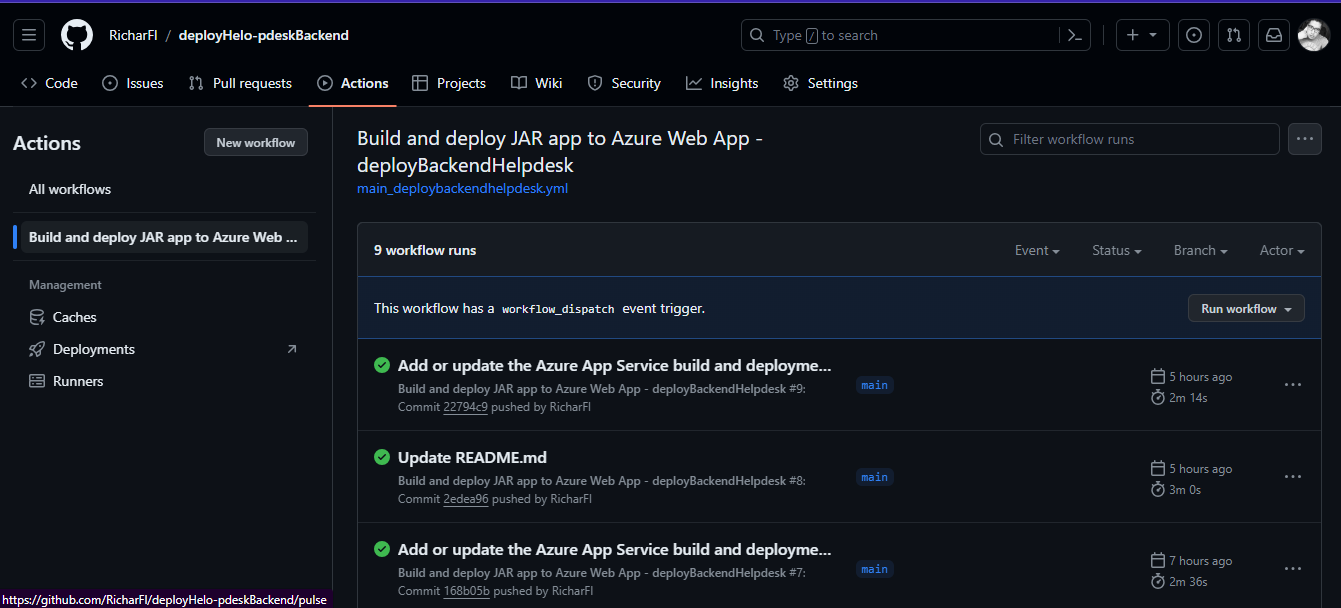
\includegraphics[width=1.1\textwidth]{CapituloImplem/Img/deploygit}
	\caption{Deploy de Sprint Boot en Repositorio de Github}
	\label{fig:deplyback}
\end{figure}

\begin{figure}[H]
	\centering
	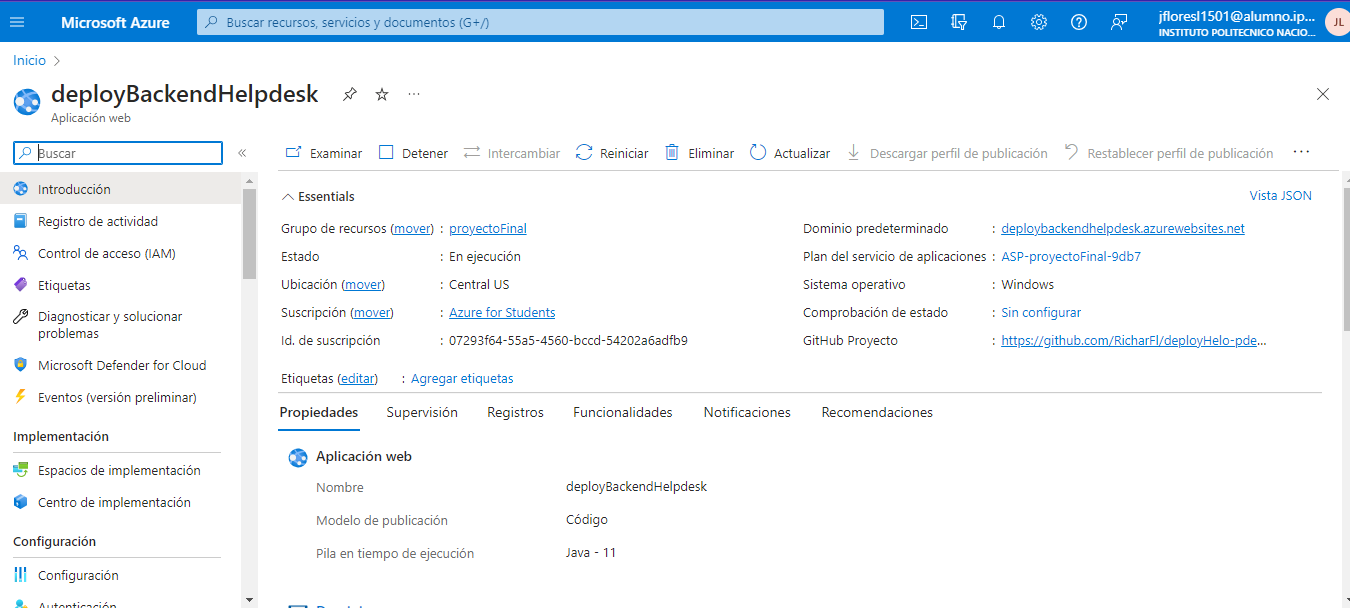
\includegraphics[width=1.1 \textwidth ]{CapituloImplem/Img/InstanciaBackenNube}
	\caption{Azure App Service "deplyBakendHelpdesk"}
	\label{fig:Azurebkacket}
\end{figure}

 
 \subsection{Despliegue de Front End en Azure }
 
 El despliegue de la instancia de Angular.js se realizo desde Visual Studio Code con su extensión  Azure App Service como se muestra en la figura \ref{fig:azureangularconf} , cabe mencionar que antes de realizar la integración con azure figura \ref{fig:ssas} ,  se tubo que haber realizado  el build del Aplicativo web. 
 \begin{figure}[H]
 	\centering
 	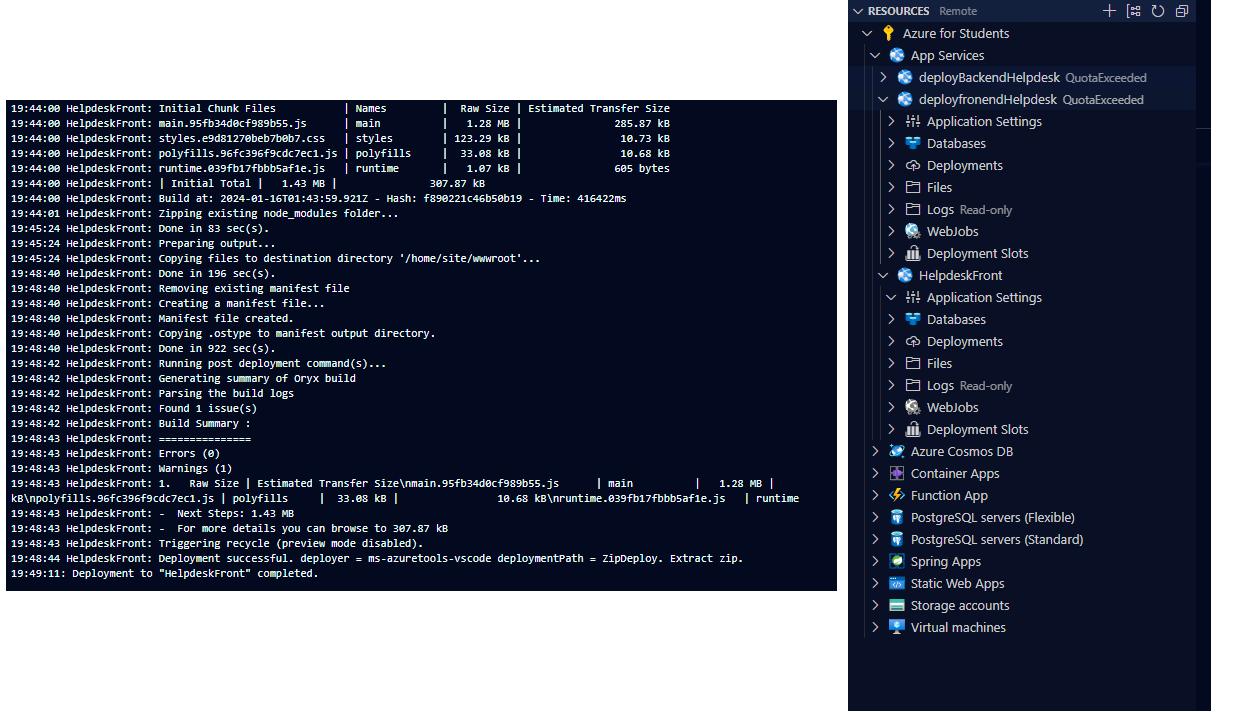
\includegraphics[width=1.1\textwidth]{CapituloImplem/Img/AngularDeploy}
 	\caption{Deploy de Angular en Visual Estudio Code y sincronizado con Azure App Service }
 	\label{fig:azureangularconf}
 \end{figure}

 \begin{figure}[H]
	\centering
	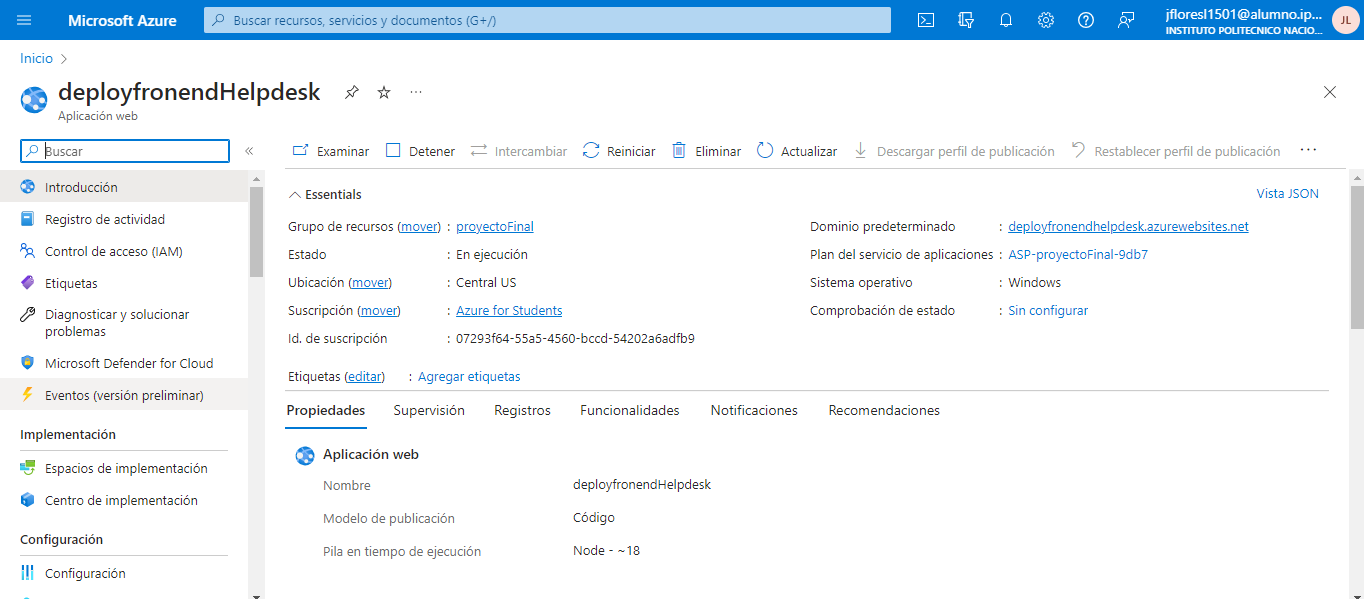
\includegraphics[width=1.1\textwidth]{CapituloImplem/Img/InstanciaAngularNube}
	\caption{Azure App Service "deployfronendHelpdesk"}
	\label{fig:ssas}
\end{figure}



\section{Aprovisionamiento de la base de datos tipo Mysql}
En un inicio, se aprovisionó una instancia de Mysql en Heroku, la cual es una 
plataforma de servicios de nube, esto debido a que los precios de Azure en comparación 
eran muy altos, sin embargo, al momento de integrar los servicios, se presentaban 
limitaciones en cuanto a la cantidad de conexiones que Heroku permitía, lo cual en 
consecuencia hizo que los servicios de Spring Boot fallaran. 
Dadas las circunstancias y después de una serie de pruebas, se encontró como alternativa 
a Azure Database for Mysql servers: Flexible Server, la cual también era una 
plataforma totalmente administrada, que permitía una cantidad suficiente de conexiones, 
además de contar con planes más accesibles. En la figura \ref{fig:mysqldatazure} se muestra la información del 
aprovisionamiento

 \begin{figure}[H]
	\centering
	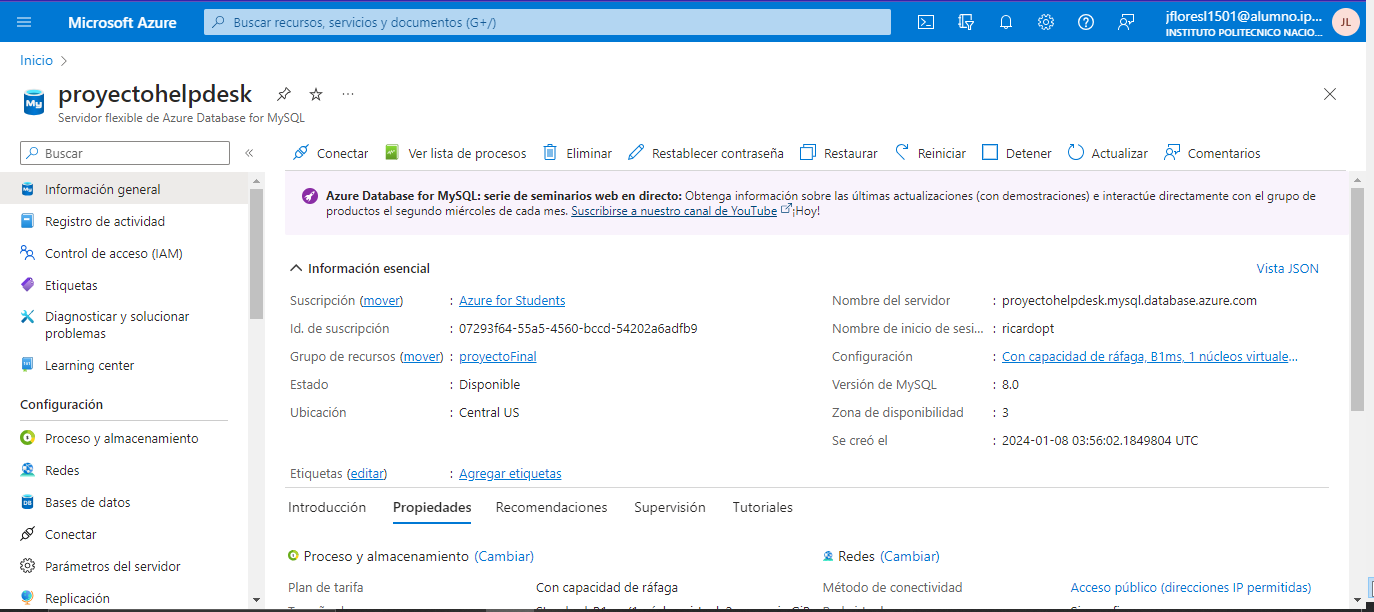
\includegraphics[width=1.1\textwidth]{CapituloImplem/Img/BasedeDatosAzue}
	\caption{Instancia aprovisionada de Azure Database for Mysql}
	\label{fig:mysqldatazure}
\end{figure}

